\renewcommand{\thechapter}{}
\renewcommand{\chaptername}{}



\section*{INTRODUCTION AND PREVIOUS WORK} 
\addcontentsline{toc}{section}{Introduction and Previous Work}

\begin{figure}[ht]
  \centering
   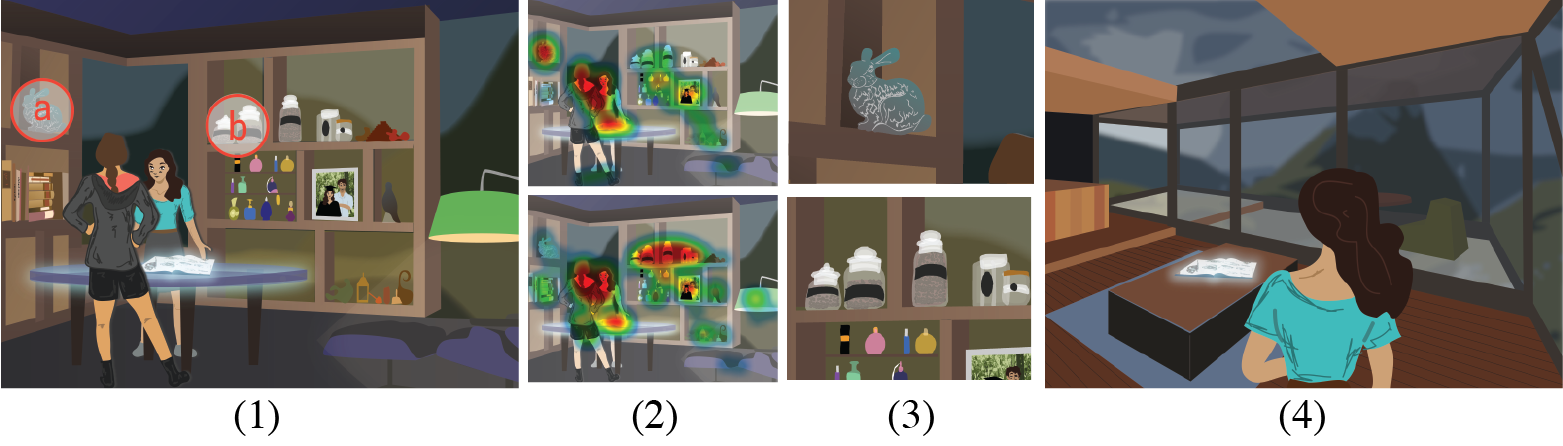
\includegraphics[height=1.7in]{figures/headerimg}
   \caption{(1) type $A$ frame with two attention elements. (2) Heat maps of user eye fixations. Top illustrates fixation on attention element a. Bottom illustrates fixation on attention element b. (3) $S$ type frames depend on varying eye gaze. (4) $K$ frame displays regardless of $S$ frame}
\end{figure}


While attention and perceptual consciousness are distinct neurobiological processes, we only consciously perceive the stimuli we attend to \citep{koch2007attention}. Attention can be allocated in a voluntary, goal-directed manner as well as captured in an involuntary, stimulus-driven manner. In both cases, eye tracking serves as a good proxy for attention \citep{hoffman1995role}. Indeed, tracking eye movements is a much better probe for attention than more indirect manual reaction time measures \citep{duc20085}.


\section*{IMPLEMENTATION} \label{chapterimplementation}
\addcontentsline{toc}{section}{Implementation}

\subsection*{Hardware and Apparatus}
\addcontentsline{toc}{subsection}{Hardware and Apparatus}

\subsection*{Framework}
\addcontentsline{toc}{subsection}{Framework}

\paragraph{Narrative Framework Representation}


We designate \textit{Frame} nodes to have 3 possible properties:
\begin{itemize}
 \setlength\itemsep{-0.5em}
 \item $K$ is a key frame and \textbf{must} appear in the narrative
 \item $S$ is a shiftable frame and \textbf{may} appear in the narrative
 \item $A$ is a frame which has attentional elements with dependent $S$ nodes
\end{itemize}


\begin{table}[h!]
  \begin{center}
    \begin{tabular}{| c || c | c |}
    \hline
    Group & Fixation Threshold Data Set & Belief State Data Set \\ \hline \hline
    Mean & 2.081410000000 & 2.137400000000 \\ \hline
    Standard Deviation (SD) & 0.437084417600 & 0.145996090400  \\ \hline
    Standard Error of the Mean (SEM) & 0.097735046966 & 0.037696028449 \\ \hline
    Population Size (N) & 20 & 15  \\
    \hline
    \end{tabular}
  \end{center}
  \caption{Average Feature Congestion Within and Among Data Sets}
\end{table}
